%Made By Thomas Debelle
\documentclass{report}
\usepackage[a4paper, total={6in, 9in}]{geometry}
\usepackage[utf8]{inputenc}
\usepackage[francais]{babel}
\usepackage{graphicx}
\usepackage{graphics}
\usepackage[T1]{fontenc}
\usepackage{amsmath}
\usepackage{hyperref}
\usepackage{amssymb}
\usepackage{listings}
\usepackage{xcolor}
\usepackage{array}
\usepackage{float}
\usepackage{amsfonts}
\usepackage{fancyhdr}
\usepackage{titlesec}
\usepackage{xparse}
\usepackage{wrapfig}

\hypersetup{
    colorlinks=true,
    linkcolor=black,
    filecolor=magenta,
    urlcolor=cyan,
    pdftitle={Overleaf Example},
    pdfpagemode=FullScreen,
    }
\begin{document}


\begin{titlepage}
    \begin{figure}
        
\includegraphics[height = 2cm]{UCL_Logo.png}
        \label{fig:my_label}
    \end{figure}

    \hspace*{100cm}
    \centering
    \vspace*{7cm}

    {\Huge \textbf{Résumé de LEPL1106}}\\
    \vspace*{0.25cm}
    compilation du \today\\
    \vspace*{0.25cm}
    \Large{Thomas Debelle}\\

    \vspace*{9.5cm}
    {\Large Juin 2023}
\end{titlepage}


\tableofcontents
\newpage

\section*{Préface}

Bonjour à toi !\\

Cette synthèse recueille toutes les informations importantes données au cours, pendant les séances de tp et est améliorée grâce au note du Syllabus. Elle ne remplace pas le cours donc écoutez bien les conseils et potentielles astuces que les professeurs peuvent vous donner. Notre synthèse est plus une aide qui, on l'espère, vous sera à toutes et tous utile.\\

Elle a été réalisée par toutes les personnes que tu vois mentionnées. Si jamais cette synthèse a une faute, manque de précision, typo ou n'est pas à jour par rapport à la matière actuelle ou bien que tu veux simplement contribuer en y apportant tes connaissances ? Rien de plus simple ! Améliore la en te rendant \href{http://www.github.com/Tfloow/Q4_EPL}{ici} où tu trouveras toutes les infos pour mettre ce document à jour. (\textit{en plus tu auras ton nom en gros ici et sur la page du github})\\

Nous espérons que cette synthèse te sera utile d'une quelconque manière ! Bonne lecture et bonne étude.


\part{Signaux}

\chapter{Les signaux}
\section{Définition}
\subsubsection{Définition}
Un signal est une fonction de une ou plusieurs variables (continues ou discrètes) qui correspondent à de l'information ou a un phénomène physique.

\subsubsection{Continues ou discrets ?}
Un signal est dit continu si il est définit sur un espace de temps continu. On note ce signal $x(t)$. Et il est dit discret si il est définit sur un espace discret de temps. On note ce signal $x[t]$.

\subsubsection{Manipulation des signaux}
Pour le cas discrets ou continu, nous pouvons réaliser les opérations suivantes.
\begin{itemize}
\item Combinaison linéaire $\rightarrow \alpha_{1}x_{1}(t) + \alpha_{2}x_{2}(t)$
\item Multiplication $ \rightarrow x_{1}[t]x_{2}[t]$
\item Dilatation $ \rightarrow x[n/a], a > \mathbb{R}$
\item Translation $ \rightarrow x(t - t_0), t_0 \in \mathbb{R}$
\item Renversement $ \rightarrow x(-t)$
\item Différentiation (que pour le cas continu) $ \rightarrow \frac{d^n x(t)}{dt^n}$
\item Intégration (que pour le cas continu)
\end{itemize}

\section{Signaux élémentaires}
\subsection{Signaux exponentiels}
Pour les signaux continus nous avons:
\begin{equation}
x(t) = B e^{at}
\end{equation}
Et pour les signaux discrets nous avons:
\begin{equation}
x[n] = Br^n \rightarrow 0 < r < 1
\end{equation}

\subsection{Signaux sinusoïdales}
Pour les signaux continus nous avons:
\begin{equation}
x(t) = A cos(\omega t + \phi)
\end{equation}
Et pour les signaux discrets nous avons:
\begin{equation}
x[n] = A cos(\Omega n + \Phi)
\end{equation}
Il a une période de $\Omega N = 2 \pi m$

\subsection{Signaux amortis}
Pour les signaux continus et avec $\alpha > 0$:
\begin{equation}
x(t) = A e^{-\alpha t}cos(\omega t + \phi)
\end{equation}
Et pour les signaux discrets:
\begin{equation}
x[n] = Br^ncos(\Omega n + \Phi)
\end{equation}

\subsection{L'impulsion (temps discret)}
Comme son nom l'indique, ce signal se représente sous la forme d'une impulsion. Par sa définition, cela nous force a avoir un signal discret !
\begin{equation}
\begin{cases}
\delta [n] = 1 \rightarrow n = 0 \\
\delta [n] = 0 \rightarrow \forall n \notin 0
\end{cases}
\end{equation}
On peut réaliser des impulsions décaler en écrivant $\delta [n-x]$ avec $x$ représentant la valeur du décalage.

\subsection{L'échelon (temps discret)}
Ce type de signal élémentaire est encore plus trivial puisqu'il se résume à:
\begin{equation}\label{eq:1}
\begin{cases}
1 \rightarrow n \geq 0 \\
0 \rightarrow n < 0
\end{cases}
\end{equation}
On peut aussi voir l'échelon comme une somme infinie d'impulsion comme $\sum_{k \geq 0}^{\infty} \delta[n-k]$.\\
Il existe également un échelon en temps continu qui se résume à la même équation \ref{eq:1} mais pour des valeurs continues.

\subsection{L'impulsion (temps continu)}
\begin{equation}
\begin{cases}
\delta (t) = 0 si t \neq 0\\
\delta (0) = ?(+\infty)\\
\int_{-a}^a \delta (s) ds = 1 \rightarrow \forall a > 0
\end{cases}
\end{equation}
A noter que la dernière ligne nous crée une propriété bien spécifique. En effet, la valeur de l'impulsion est limité par les bornes $a$ puisqu'on impose une intégrale égale à 1.

\subsubsection{Lien entre impulsion et échelon}
$\delta (t) = u'(t)$ donc l'impulsion est une sorte de dérivé de l'échelon. ceci nous permet également d'obtenir cette formule:
\begin{equation}
\int_{-\infty}^{\infty} x(s) \delta(s)ds = x(0)
\end{equation}
On prouve cela de manière \textit{peu rigoureuse} en remarquant que: pour $s \neq 0$, on a $\delta(s) = 0$ donc $x(s)\delta(s) = 0 = x(0)\delta(s)$ finalement on a:
\begin{equation}
\int_{-\infty}^{\infty} x(s) \delta(s)ds = \int_{-\infty}^{\infty} x(0) \delta(s)ds = x(0) \int_{-\infty}^{\infty} \delta(s)ds = x(0)
\end{equation} 

\subsubsection{Décomposition en impulsions}
On peut décomposer tout signal en impulsion comme ci-dessous:
\begin{equation}
\begin{cases}
\text{temps discret } \Rightarrow x[n] = \sum_{k=-\infty}^{\infty}x[k]\delta[n-k] \\
\text{temps continu } \Rightarrow x(t) = \int_{-\infty}^{infty} x(s) \delta(t-s)ds
\end{cases}
\end{equation}



\section{Convolution} \label{convo}
La convolution est une nouvel opérateur qui nous sera très utile. Son signe est "$\ast$" et la formule qui définit cette opération est:
\begin{equation}
f[n] \ast g[n] := \sum_{k=-\infty}^{\infty} f[k]g[n-k] 
\end{equation}
La méthode pour trouver le résultat d'une convolution est:
\begin{enumerate}
\item Il faut "\textit{renverser}" une des fonctions. C'est-à-dire faire $f[n] \rightarrow f[-n]$.
\item Puis multiplier ces deux nouvelles fonctions.
\item L'\textit{aire} sous la courbe créer par cela est le résultat de la convolution.
\end{enumerate}

\chapter{Fourier}
\section{La représentation de Fourier}

\subsection{Signaux continus}
\subsubsection{Stocker un signal efficacement}
Un signal est composé de sinus et de cosinus à des amplitudes, phases et fréquences différentes.\\
La manière la plus efficace pour stocker un signal est d'avoir pour chaque fréquence \textit{multiple} de la fréquence de base $\omega_0$ son amplitude. (on verra que en effet, on peut faire cette supposition que chaque fréquence sont des multiples fréquences) Cela ressemble donc à ça:
\begin{align}
x(t) &= \textcolor{red}{1}cos(\textcolor{red}{1}\omega_0t) + \textcolor{blue}{2}sin(\textcolor{blue}{2}\omega_0t) + \textcolor{red}{\frac{1}{2}}cos(\textcolor{red}{2}\omega_0t) + \textcolor{blue}{\frac{1}{2}}sin(\textcolor{blue}{3}\omega_0t) +  \textcolor{red}{\frac{4}{5}}cos(\textcolor{red}{4}\omega_0t) \label{eq:signal}\\
cos &= [\textcolor{red}{1}, \textcolor{red}{\frac{1}{2}}, \textcolor{red}{0}, \textcolor{red}{\frac{4}{5}}]\\
sin &= [\textcolor{blue}{0}, \textcolor{blue}{2}, \textcolor{blue}{3}]
\end{align}
\subsubsection{Périodicité}
On sait que $x(t)$ est \textcolor{blue}{périodique} et d'\textit{énergie finie}.(Périodicité de $\omega_0 = \frac{1}{T_0}$ Pour décomposer notre signal en \textbf{Série de Fourier \textit{trigonométrique}}:
\begin{align}
x(t) &= a_0 + \sum_{k=1}^{+\infty} \Bigl(2 a_k cos(k\omega_0 t) + 2b_k sin(k \omega_0 t) \Bigl)\\
a_k &= \frac{1}{T_0} \int_0^{T_0} x(t) cos(k\omega_0t)dt\\
b_k &= \frac{1}{T_0} \int_0^{T_0} x(t) sin(k\omega_0t)dt
\end{align}
De plus, on peut toujours décomposé un signal \textit{périodique} en une partie \textbf{impaire} et \textbf{paire}. (en fourier, il suffit de prendre la partie cos donc paire et sin donc impaire)\\

Chose importante à remarquer, on va souvent tracer des graphes avec un axe y de type $2a[n]$. Ce 2 est un des prémices de Fourier complexe.

\subsubsection{Signaux carrés}
Un signal carré est de type avec une période de $2\pi$:
\begin{align}
x(t) = \begin{cases}
1 \qquad &\text{si } 0 \leq t < \pi\\
-1 \qquad &\text{sinon}
\end{cases}
\end{align}
Si on fait la série de Fourier, on peut se rendre compte que ce signal est composé d'une \textit{infinité} de sinus de tel sorte que:
\begin{equation}
x(t) = \sum_0^{+\infty} \frac{1}{2n+1} sin((2n+1)t)
\end{equation}

\subsubsection{Fourier Complexes}
On voit que cette série est bien plus simple et est une révolution pour calculer \textit{Fourier}:
\begin{align}
x(t) &= \sum_{k = - \infty}^{+ \infty} X_k e^{jk\omega_0 t}\\
X_k &= \frac{1}{T_0} \int_0^{T_0} x(t) e^{-jk\omega_0t}dt \label{eq:coefComplexe}
\end{align}
Donc on prend le conjugué pour calculer $X_k$. C'est ici que le coefficient $2$ fait du sens, on se rappelle les formules d'Euler.
\begin{equation}
cos(t) = \frac{e^{jt} + e^{-jt}}{2} \qquad \qquad sin(t) = \frac{e^{jt} - e^{-jt}}{2j}
\end{equation}
Donc le lien avec la série en Réelle est: $X_0 = a_0$, $X_k = X_{-k}^{*} = a_k -jb_k$. On trouve cela en injectant dans l'équation \ref{eq:coefComplexe} la formule d'Euler.

\subsubsection{Représentation de Fourier} %télécharger les images des slides à jour
Pour faire la représentation de Fourier, on va commencer par prendre l'équation \ref{eq:signal} et la transformer:
\begin{align}
x(t) &= 2(\textcolor{red}{\frac{1}{2}}cos(\textcolor{red}{1}\omega_0t) + \textcolor{red}{\frac{1}{4}}cos(\textcolor{red}{2}\omega_0t) + \textcolor{red}{\frac{4}{10}}cos(\textcolor{red}{4}\omega_0t)) + 2(\textcolor{blue}{1}sin(\textcolor{blue}{2}\omega_0t)  + \textcolor{blue}{\frac{1}{4}}sin(\textcolor{blue}{3}\omega_0t)) \label{eq:signalT}
\end{align}
Ensuite on injecte la formule d'Euler dans l'équation \ref{eq:signalT} ce qui donne:
\begin{figure}[H]
\centering
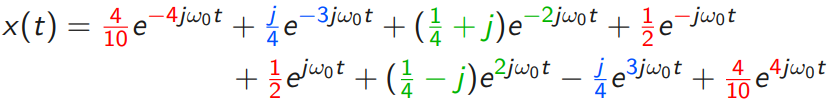
\includegraphics[width=8cm]{img/signalTE.png} %oui c'est une photo donc si quelqu'un est chaud ré-écrire proprement l'équation
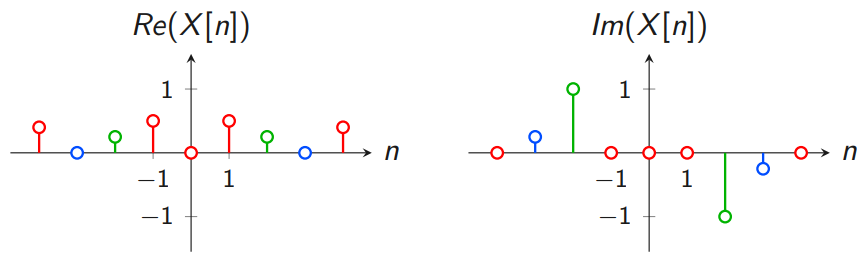
\includegraphics[width=6cm]{img/grapheSignalTE.png}
\end{figure}
Notre signal $x(t)$ est bien défini de manière unique via ses coefficients !


\subsubsection{Base orthogonale}
Les exponentielles complexes de Fourier sont orthogonales dans l'espace de Hilbert $\mathcal{H}_T$ équipé avec le produit scalaire:
\begin{align}
\langle x, y\rangle &= \frac{1}{T_0}\int_0^{T_0}x(t)y^{*}(t)dt\\
\{e^{jk\omega_0t}\}&, k \in \mathbb{Z} \rightarrow \textbf{ est }\perp
\end{align}

\subsection{Signaux discrets}
La périodicité d'un signal change puisqu'on ne peut avoir que des valeurs $\mathbb{N}$. En effet, on dit qu'un signal est de période N si $x[n + N] = x[n]$. De plus, N est en $[rad]$ et pas $[\frac{rad}{s}]$ car la \textcolor{blue}{pulsation fondamentale} est $\Omega_0 = \frac{2\pi}{N}$

\subsubsection{Calcul de la série de Fourier}
\begin{align}
x[n] &= \sum_{k=0}^{N-1} X[k] e^{jk\Omega_0n}\\
X[k] &= \frac{1}{N} \sum_{m=0}^{N-1} x[m] e^{-jk\Omega_0m}
\end{align}
On a seulement besoin de $N$ coefficient grâce à la \textbf{périodicité}. En effet, $e^{j(N+k)\Omega_0n} = e^{jk\Omega_0n}$



\section{La transformée de Fourier}
Cela s'applique sur les signaux \textit{non-périodiques} et \textit{continus}.\\
Il faut donc voir le signal comme ayant un $\omega = 0 = \frac{1}{T_0} = \frac{1}{\infty}$ et y appliquer la série de Fourier!

\subsection{Calcul de la transformée}
On dit que le \textcolor{blue}{spectre} $X(j\omega)$ du signal $x(t)$ est sa \textbf{transformée de Fourier}.
\begin{align}
X(j\omega) &= \int_{-\infty}^{\infty} x(t) e^{-j \omega t}dt\\
x(t) &= \frac{1}{2\pi} \int_{-\infty}^{\infty} X(j\omega) e^{j\omega t} d\omega \label{eq:invF}
\end{align}
On appelle l'équation \ref{eq:invF}, la transformée de Fourier \textbf{inverse}.\\

Pour arriver ce résultat, nous avons réaliser quelque modification à la série de Fourier:
\begin{align}
\omega_k &= k \omega_0 = \frac{2 \pi k}{T_0} \Rightarrow \omega_{k+1} - \omega{k} = \Delta \omega = \frac{2\pi}{T_0}\\
\int_0^{T} & \approx \int_{\frac{-T}{2}}^{\frac{T}{2}} \qquad \text{ Pour "couvrir" tout le domaine}\\
x(t) &= \sum_{-\infty}^{\infty} X_k e^{j \omega_0 k t}\\
	 &= \sum_{-\infty}^{\infty} \Bigl \{ \frac{1}{T_0} \int_{\frac{-T_0}{2}}^{\frac{T_0}{2}} x(t) e^{-j k \omega_0 t} dt \Bigl \} e^{j k \omega_0 t}\\
	 &= \sum_{-\infty}^{\infty} \frac{1}{2 \pi} \int_{\frac{-T_0}{2}}^{\frac{T_0}{2}} x(t) e^{-j k \omega_0 t} dt\quad e^{j k \omega_0 t} \Delta \omega \label{eq:finalF}
\end{align} 
On remarque qu'on a 2 parties intéressantes dans l'équation \ref{eq:finalF}. On a une partie qui évolue dans le temps, c'est notre \textit{signal continu}, c'est notre \textcolor{blue}{spectre}. L'autre partie dépend de la fréquence et c'est la \textit{reconstruction du signal}. 
\begin{figure}[H]
\centering
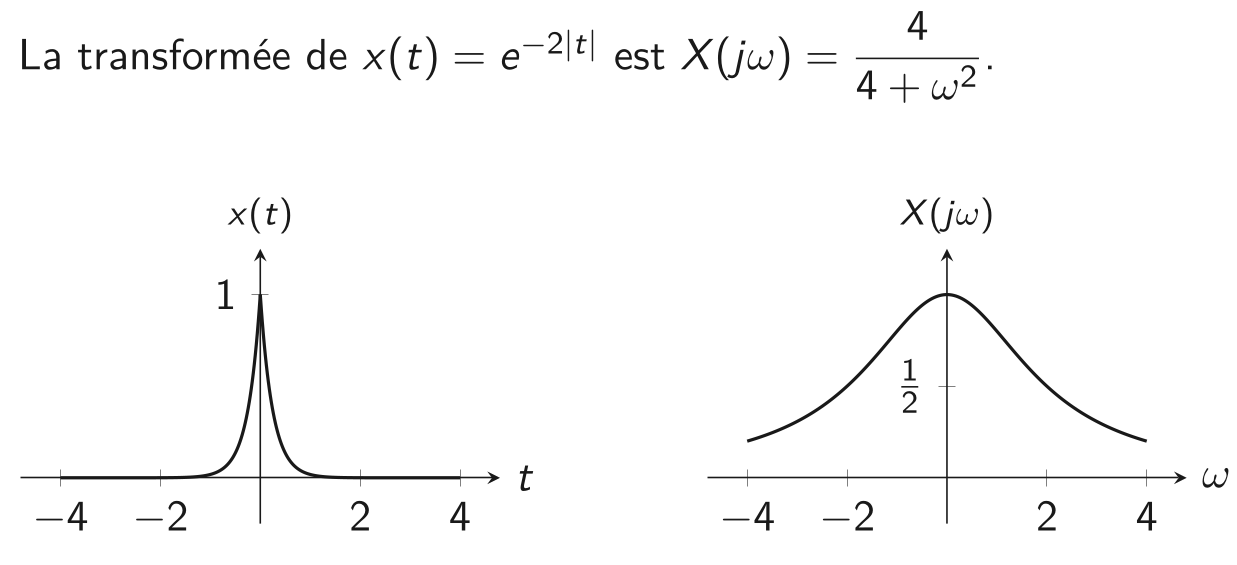
\includegraphics[width=7cm]{img/reconstructionF.png}
\caption{à gauche, un signal pair \qquad à droite, le spectre}
\end{figure}

\subsection{Calcul discret}
On a un signal $x[n]$ qui s'exprime de manière unique selon ses fréquences:
\begin{align}
x[n] &= \frac{1}{2\pi}\int_{-\pi}^{\pi} X \bigl(e^{j\Omega} \bigl) e^{j\Omega n} d\omega\\
X\bigl(e^{j\Omega} \bigl) &= \sum_{m=-\infty}^{\infty} x[m]e^{-j\Omega m} \label{eq:transfoDF}
\end{align}
L'équation \label{eq:transfoDF} donne la \textcolor{blue}{transformée} de Fourier.


\part{Systèmes}

\chapter{Système LIT}
Un système est une entité qui prend \textit{un ou plusieurs signaux} en entrée et produit \textit{de nouveaux signaux} en sortie.\\
Exemple: $H\{x[n]\} = x[n] + x[n-1]$. Un système est par exemple: \textit{une radio, une caméra, une voiture, ...}

\section{LIT}
Un système \textit{Linéaire et Indépendant du Temps} ou \textbf{LIT} est, comme son nom l'indique, linéaire donc:
\begin{equation}
\mathcal{H}\{a_1x_1 + ... + a_Nx_N\} = a_1\mathcal{H}\{x_1\} + ... + a_N\mathcal{H}\{x_N\} 
\end{equation}
Et un système est \textit{invariant temporelle} donc:
\begin{equation}
\begin{cases}
\mathcal{H} \text{ est invariant si } \forall t_0 \in \mathbb{N}\\
\mathcal{H}\{x\}[n] = y[n] \Rightarrow \mathcal{H}\{x[n-n_0]\} = y[n-n_0]
\end{cases}
\end{equation}
On remarque qu'on peut ré-écrire tous signaux via une somme d'impulsions. De plus, si $\mathcal{H}$ est linéaire alors:
\begin{equation}
\mathcal{H}\{x\} = \mathcal{H}\biggl\{\sum_{k= -\infty}^{\infty} x[k]\delta[n-k] \biggl\} = \sum_{k=-\infty}^{\infty} x[k]\mathcal{H}\{\delta[n-k]\}
\end{equation}
Si $\mathcal{H}$ est \textit{invariant} au temps et qu'on pose $h := \mathcal{H}\{\delta\}$
\begin{align}
\mathcal{H}\{\delta[n-k]\} = \mathcal{H}\{\delta\}[n-k] &= h[n-k]\\
\mathcal{H}\{x\} = \sum_{k=-\infty}^{\infty} x[k]h[n-k] &=: x \ast h
\end{align}
A noter que "$\ast$" fais référence à la convolution, sujet abordé à la section \ref{convo}.\\

Il est important de noter que toutes ces propriétés et caractéristiques des systèmes \textit{LIT} en \textbf{temps discret} sont également valables et ont un équivalent en \textbf{temps continu}.



\section{Opération sur les signaux}
Voici un tableau résumant les différentes opérations possibles sur les signaux:
\begin{center}
\begin{tabular}{|c|c|c|}
	\hline
	 & Temps discret & Temps continu\\
	\hline
	Combinaison linéaire & $\alpha_1 x_1[n] + \alpha_2 x_2[n]$ & $\alpha_1 x_1(t) + \alpha_2 x_2(t)$\\
	\hline
	Multiplication & $x_1[n]x_2[n]$ & $x_1(t)x_2(t)$\\
	\hline
	Différentiation &  & $d^nx(t)/dt^n$\\
	\hline
	Intégration &  & $\int_{-\infty}^t x(\tau)d\tau$\\
	\hline
	\textbf{Convolution} & $x_1[n] \ast x_2[n]$ & $x_1(t) \ast x_2(t)$\\
	\hline
	Dilatation & $x[n/a]$ (arrondi $n/a$) & $x(t/a) a>0$\\
	\hline
	Translation & $x[n-n_0], n_0 \in \mathbb{Z}$ & $x(t-t_0), t_0 \in \mathbb{R}$\\
	\hline
	Renversement & $x[-n]$ & $x(-t)$\\
	\hline
\end{tabular}
\end{center}
Une chose importante à voir dans ces formules est que $x$ est un \textit{signal}, $x[k]$ la \textit{valeur} de ce signal en k et on a $\mathcal{H}$ qui est un \textit{système} prenant et donnant des signaux.

\section{Convolution (temps discret)} \label{convo}
La convolution est un nouvel opérateur qui nous sera très utile. Son signe est "$\ast$" et la formule qui définit cette opération est:
\begin{equation} \label{eqn:convolution}
f[n] \ast g[n] := \sum_{k=-\infty}^{\infty} f[k]g[n-k] 
\end{equation}
La méthode pour trouver le résultat d'une convolution de manière \textbf{graphique} est:
\begin{enumerate}
\item Il faut "\textit{renverser}" une des fonctions. C'est-à-dire faire $f[n] \rightarrow f[-n]$.
\item On décale une des fonctions le plus à droite. (on prend le $k_0$ où après, tous les résultats de $f[k]g[n-k]$ valent $0$) 
\item Puis multiplier chaque point entre eux et les sommer.
\item On met le résultat sur un \textit{graphe} au point $k$.
\item On décale notre fonction d'un point vers la gauche et on répète le processus.
\end{enumerate}
Pour trouver de manière \textbf{calculatoire}, on applique simplement la formule \ref{eqn:convolution}.

\subsection{Propriétés}
\begin{center}
\begin{tabular}{c|c}
	Commutativité & $(f\ast g)[n] = (g \ast f)[n]$ \\
	\hline
	Associativité & $(f \ast (g \ast h))[n] = ((f \ast g) \ast h)[n]$ \\
	\hline
	Distributivité & $(f \ast (g + h))[n] = (f \ast g + f \ast h)[n]$ \\
\end{tabular}
\end{center}
On également ces propriétés:
\begin{center}
\begin{tabular}{c|c}
	Élément neutre & $f[n] \ast \delta[n] = f[n]$ \\
	\hline
	Décalage & $f[n] \ast \delta[n-n_0] = f[n-n_0], n_0 \in \mathbb{Z}$ \\
\end{tabular}
\end{center}

\section{Convolution (temps continu)}
Cette formule ressemble très fort à celle vu en temps continu à la section \ref{convo}. Si on a \textit{2 signaux} $f(t)$ et $g(t)$ leur convolution est donnée par:
\begin{equation}
f(t) \ast g(t) = \int_{-\infty}^{\infty}f(\tau)g(t-\tau)d\tau
\end{equation}
Pour calculer de manière \textbf{graphique} il faut suivre ces étapes:
\begin{enumerate}
\item Il faut "\textit{renverser}" une des fonctions. C'est-à-dire faire $f(t) \rightarrow f(-t)$.
\item On décale une des fonctions le plus à droite. (on prend le $\tau_0$ où après, tous les résultats de $f(t)g(t-\tau_0)$ valent $0$) 
\item Puis multiplier chaque point entre eux et on les intègre. (on prend la surface sous la courbe).
\item On met le résultat sur un \textit{graphe} au pont $\tau$.
\item On décale notre fonction d'une distance (pas trop loin mais pas trop proche pour ainsi avoir une nuée de points) vers la gauche et on répète le processus.
\end{enumerate}
En somme, nous avons une méthode très proche du temps discret si ce n'est l'utilisation d'intégrale allant de $-\infty$ à $\infty$.

\subsection{Propriétés}
On retrouve les mêmes propriétés que en temps discret.
\begin{center}
\begin{tabular}{c|c}
	Commutativité & $(f\ast g)(t) = (g \ast f)(t)$ \\
	\hline
	Associativité & $(f \ast (g \ast h))(t) = ((f \ast g) \ast h)(t)$ \\
	\hline
	Distributivité & $(f \ast (g + h))(t) = (f \ast g + f \ast h)(t)$ \\
\end{tabular}
\end{center}
On également ces propriétés:
\begin{center}
\begin{tabular}{c|c}
	Élément neutre & $f(t) \ast \delta(t) = f(t)$ \\
	\hline
	Décalage & $f(t) \ast \delta(t-t_0) = f(t-t_0), n_0 \in \mathbb{R}$ \\
\end{tabular}
\end{center}

\section{Réponse impulsionnelle}
La réponse impulsionnelle d'un système \textit{LIT} $\mathcal{H}$ est la réaction du système à une \textit{impulsion d'entrée} ($\delta[0]$) on le note $h$.\\

Pour \textbf{tout} système \textit{LIT}, le signal de sortie est le résultat de la convolution entre \textit{le signal d'entrée} et \textit{la réponse impulsionnelle}.
\begin{align}
y[n] &= x[n] \ast h[n]\\
y(t) &= y(t) \ast h(t)
\end{align}

\section{Type de système}
\begin{center}
\begin{tabular}{|c|c|}
	\hline
	Système sans mémoire & Si la sortie du système \textit{à un temps donné}\\
	&  ne dépend que de l'entrée à \textbf{cet instant}.\\
	\hline
	Système causal & Le système \textbf{ne dépend pas} de ce qui se passe dans le \textit{futur}\\
	\hline
	Système stable ou (\textit{BIBO}) & Entrée \textit{bornée} donne une sortie \textit{bornée}\\
	\hline
	Système inversible & On sait \textit{retrouver} l'entrée en ayant la \textit{sortie}.\\
	\hline

\end{tabular}
\end{center}

\section{Modélisation et représentation des systèmes}
Comme vu précédemment, la réponse impulsionnelle est le résultat du système étant perturbé par une impulsion. 
\subsection{Inconvénient}
\begin{enumerate}
\item Fonction de taille \textit{infinie} et représentation donc \textit{peu simple}.
\item La modélisation d'un système ne mène généralement pas à une réponse impulsionnelle .
\item On doit connaitre l'entrée depuis $-\infty$
\end{enumerate}


\subsection{Représentation}
\begin{wrapfigure}{r}{.3\textwidth}
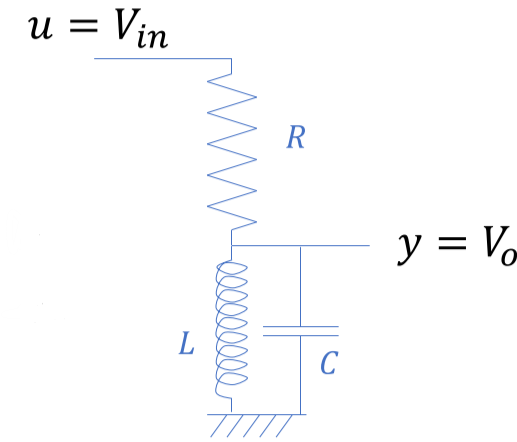
\includegraphics[width=5cm]{img/RLC.png}
\caption{Circuit RLC}
\label{fig:RLC}
\end{wrapfigure}
Il existe 3 grandes façons de représenter un système. Tout d'abord la méthode \textit{équation différentielle d'entrée-sortie}. Pour la suite des exemples, j'utiliserai un circuit \textit{RLC} comme montré ci-contre.\\

\textit{équation différentielle d'entrée-sortie} est une somme des dérivées comme montré dans l'équation \ref{eqn:es}. C'est plutôt facile de trouver les équations mais on fait face à un problème, l'opération \textit{dérivée} n'existe pas dans le monde réelle, il faut un opérateur intégrateur.\\

Ensuite, nous avons la \textit{représentation d'état} qui utilise des matrices pour former les équations différentielles comme nous voyons à l'équation \ref{eqn:mat}\\

La dernière représentation type est le \textit{schéma bloc} qui est visuel et qui utilise lui des blocs intégrateurs au lieu de dérivé comme montré à la figure \ref{fig:bloc}.

\begin{equation} \label{eqn:es}
\ddot{y} + \frac{1}{CR}\dot{y} + \frac{1}{LC}y = \frac{1}{CR}\dot{u}
\end{equation}

\begin{equation} \label{eqn:mat}
\frac{d}{dt}\begin{pmatrix}
V_0\\
I_L
\end{pmatrix} = \begin{pmatrix}
-1/RC & -1/C\\
1/L & 0
\end{pmatrix} \begin{pmatrix}
V_0\\
L
\end{pmatrix} + \begin{pmatrix}
1/RC\\
0
\end{pmatrix} u
\end{equation}

\begin{figure}[H] 
\centering
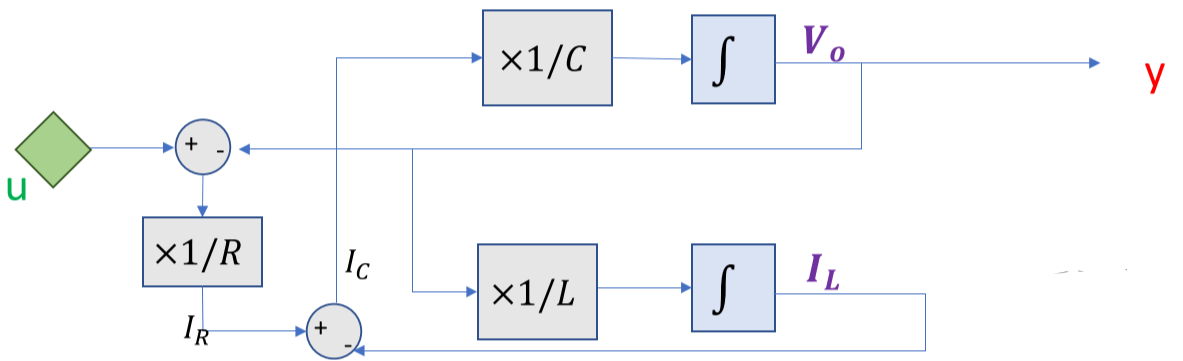
\includegraphics[width=7cm]{img/bloc.png}
\caption{Repésentation \textit{bloc} du système à la figure \ref{fig:RLC}}
\label{fig:bloc}
\end{figure}

\subsection{Équation différentielle entrée-sortie}
La forme générale de ces équations est de ce type:
\begin{equation}\label{eqn:difes}
\sum_{k = 0}^{N} a_k (\frac{d^k}{dt^k}) y(t) = \sum_{k = 0}^M b_k (\frac{d^k}{dt^k}) u(t)
\end{equation}
Quelque chose à bien remarquer est que ces équations ne modélise \textit{qu'une partie} d'un système \textit{LIT}. Par exemple, on ne peut pas représenter un \textit{délai} ce qui également rare dans la réalité.\\

Une chose à remarquer est que l'opérateur \textit{dérivé} peut se "\textit{démultiplier}" et possède une \textit{associativité} et \textit{commutativité}. Ainsi, on peut avoir une représentation dite "\textit{polynomiale}" comme ci-dessus qui est une autre écriture de l'équation \ref{eqn:difes}.
\begin{equation}\label{eqn:poly}
p(\frac{d}{dt})y(t) = q (\frac{d}{dt})u(t)
\end{equation}
Puis après, pour résoudre ce genre d'équation, on utilise des méthodes classiques vu au cours d'Analyse donc, solution homogène et particulière ...

\subsubsection{Réponse libre et forcée}
Une réponse \textit{libre} est la solution de l'équation homogène, donc quand $u(t) = 0$ à l'équation \ref{eqn:poly} et on garde les \textbf{mêmes conditions initiales}. En somme c'est la représentation de l'impact des \textit{CI}.\\

Une réponse \textit{forcée} est l'équation \ref{eqn:poly} mais avec les \textit{conditions initiales} nulles. Donc on s'intéresse à l'impact de l'entrée sans les conditions initiales. La somme de la réponse \textit{libre} et \textit{forcée} nous donne la réponse générale.

\subsubsection{Stabilité}
On peut avoir une intuition sur la stabilité de notre système en posant $y_H(t)$ qui équivaut à:
\begin{equation}
y_H(t) = \sum_i \alpha_ie^{r_it} \rightarrow \quad r_i \text{ correspond aux racines de p(z) de \ref{eqn:poly}}
\end{equation}
Si la partie réelle de $r_i < 0 \forall i$ alors on a une exponentielle décroissante donc \textbf{stable}. On appelle ce genre de système \textit{BIBO} stable ou \textit{Bounded Input Bounded Output}.\\

En revanche, si $r_i > 0 \exists i$ donc on a au moins une exponentielle croissante créant une \textit{instabilité}.\\

Si $r_i = 0 \exists i$ on dit qu'on a une \textit{stabilité marginale} ou \textit{instabilité}. Cela dépendera de la \textbf{multiplicité} et de \textbf{$te^{r_it}$}.

\subsubsection{Linéarité de l'entrée}
Avec cette représentation polynomiale, on peut facilement voir qu'on a une linéarité de l'entrée nous permettant de simplifier différent calcul. %rajouter la formule etc

\subsubsection{Avantages et Inconvénients}
2 représentations qui sont \ref{eqn:difes} et \ref{eqn:poly}. Les avantages:
\begin{itemize}
\item Représentation compacte.
\item Conditions initiales claires.
\item Facile de la transformer dans d'autres représentations.
\end{itemize}
Les désavantages:
\begin{itemize}
\item On peut perdre la représentation physique.
\end{itemize}

\subsection{Schéma Bloc}
Comme son nom l'indique, le schéma bloc utilise des "\textit{blocs}" pour représenter notre système. Ci-dessus on peut voir les composants de base composant ce type de schéma
\begin{figure}[H]
\centering
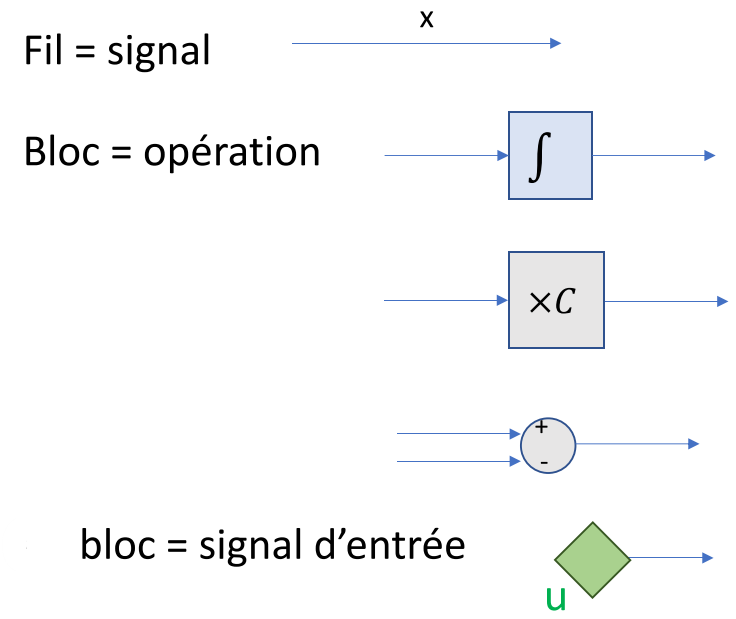
\includegraphics[width=5cm]{img/blocExemple.png}
\caption{Liste reprenant les blocs de base}
\end{figure}
Dans le cadre des systèmes \textit{LIT}, on se restreint souvent à l'addition, multiplication et intégration. On ne réalise que des opérations \textit{linéaires}.

\subsubsection{Avantages et Inconvénients}
Les avantages:
\begin{itemize}
	\item Représentation très intuitive.
	\item Proche de l'implémentation réelle du système.
	\item On peut plus facilement réfléchir sur le \textit{design} de notre système.
	\item Très modulaire.
\end{itemize}
Les désavantages:
\begin{itemize}
	\item Lien moins clair avec la solution.
\end{itemize}
De plus, on peut voir comme un \textit{avantage} ou \textit{inconvénient} le fait de pouvoir voir l'évolution des signaux entre chaque bloc plutôt qu'une sorte de boite noire "\textit{entrée-sortie}". De plus, on peut réaliser de bien des manières des circuits.

\subsection{Représentation d'état}
Dans ce type de représenation, on a \textcolor{red}{état $x$} qui est un \textit{vecteur} comportant toutes les infos internes de notre système. On \textcolor{red}{entrée $u$} qui est un \textit{signal} extérieur affectant le système. Finalement on a une \textcolor{red}{sortie $y$} qui est un signal qu'on peut accéder depuis l'extérieur.\\
\begin{equation}
\begin{cases}
\text{évolution: }\frac{d}{dt}x(t) =  Ax(t) + Bu(t)\\
\text{sortie: } C x(t) + D u(t)
\end{cases}
\end{equation}

\subsubsection{Solution}
La solution \textit{homogène} de $e^{\lambda_it}$ avec $\lambda_i$ étant les valeurs propres de l'équation. Si la partie réelle des racines est négative pour tout $\lambda_i$.

\subsubsection{État non-unique}
Avec cette représentation, on peut facilement modifier les vecteurs et signaux pour rendre les équations plus simples. Cela n'a aucun impacte et rend les équations plus logiques pour un certain sens "\textit{réel}".
\begin{equation} \label{eqn:nonunique}
\begin{cases}
z = Tx \Rightarrow \frac{d}{dt}z = T\frac{d}{dt}x = TAT^{-1}z(t) + TBu(t)\\
y = Cx(t) + Bu(t) = CT^{-1}z(t) + Du(t) 
\end{cases}
\end{equation}

Si la matrice $A$ est diagonalisable, on peut réaliser un \textbf{découplage} et obtenir ainsi un mode dit \textit{découplé}. On peut également faire des \textit{blocs de Jordan} pour diagonaliser le tout:
\begin{equation}
\frac{d}{dt} z_i = \lambda_i z_i + \tilde{B}_i u
\end{equation}

\subsection{Passage de représentation}
% à faire et ajouter les graphes
\subsection{Temps discret}
Pour passer du temps continu au temps discret, il faut transformer $\frac{d}{dt}$ en l'opérateur de \textit{décalage} $D$:
\begin{equation}
Dx[n] =  x[n-1]
\end{equation}
Ce qui nous permet d'établir l'équation de \textit{différence}
\begin{equation}
\begin{cases}
\sum_{k=0}^N a_k y[n-k] = \sum_{k=0}^M b_ku[n-k]\\
p(D)y = q(D)u
\end{cases}
\end{equation}
Ce qui nous donne pour solution homogène:
\begin{equation}
y_H [N] = \sum_i c_i r_i^n
\end{equation}
On a une décroissance donc \textit{stabilité} si $|r_i| < 1$ et une croissance si $|r_i| > 1$\\
De plus, on remplace le bloc \textit{intégrateur} du temps discret en bloc $D^{-1}$. La ré-écriture de l'équation \ref{eqn:nonunique} en temps discret:
\begin{equation}
\begin{cases}
x[n+1] = Ax[n] + Bu[n]\\
y[n] = Cx[n] + Du[n]
\end{cases}
\end{equation}
On approxime un système en temps \textit{continu} en temps \textit{discret} ssi:
\begin{equation}
A_d \approx A_c \Delta t \text{ si } \Delta t \text{ petit}
\end{equation}

\subsection{Résumé}
\begin{enumerate}
\item Réponse impulsionnelle, universelle mais peu maniable $\Rightarrow$ On voit que l'entrée et sortie et \textbf{Pas de CI}
\item Équation différentielle entrée-sortie $\Rightarrow$ On voit que l'entrée et sortie et on a des \textbf{CI}
\item Représentation d'état (matrice) $\Rightarrow$ On voit l'intérieur et on a des \textbf{CI}
\item Schéma Bloc (très concret) $\Rightarrow$ On voit l'intérieur et on a des \textbf{CI}
\end{enumerate}

\subsection{Existence des systèmes LIT}
Une forme usuelle des systèmes LIT dans la vraie vie est de type $\dot{x}(t) = f(x(t), u(t), t)$.\\
\textbf{Invariance temporelle}: tout système fait face à l'usure mais on estime que sur la période d'observation, l'usure est minime et peut être ignorée.\\
\textbf{Linéarité}: aucun système n'est pas linéaire. Cela peut être dû à des \textit{imperfections} ou si on augmente \textit{énormément} l'entrée ce qui change le comportement du système.\\



\end{document}
